\documentclass[handout]{beamer}

%load any additional packages

\usepackage[utf8]{inputenc} % so we can input characters with accents (e.g. ő)

\usepackage{mathtools}

\usepackage{gtbeamer}

\usepackage{graphicx} % ease graphics management
\graphicspath{{images/}} % define folder with images
\usefonttheme{serif} % change font to allow \textbf{}
\usepackage{palatino} % Nicer fonts
\usepackage[ruled]{algorithm2e}
\usepackage{amsmath,amsthm,amssymb} % for math equations
\usepackage{xcolor}
\usepackage{natbib} % richer citation
\usepackage{breakcites} % avoid overfull hbox for long cites

% \theoremstyle{claim}
\newtheorem{claim}[theorem]{Claim}%
\newtheorem{proposition}[theorem]{Proposition}
\setbeamertemplate{footline}[frame number]
\newcommand\norm[1]{\lVert#1\rVert}
% \newcommand\normx[1]{\lVert#1\rVert_{#2}}
\setbeamertemplate{headline}{}

% \usetheme{Szeged}

%% Information (author, title, etc.) %%

\title[PMD]{% short title for footer
    Reinforcement Learning and \\Policy Mirror Descent\\ an introduction
    \vspace{0.5cm}
}

\author{Feiyang Wu}

\institute{
        \textit{College of Computing, School of Computer Science}\\
        \textit{Georgia Institute of Technology}
        \vspace{0.5cm}
}
\date[\today]{
    \today
}

\begin{document}

% Title slide %
{
    \setbeamertemplate{footline}{}
    \setbeamertemplate{headline}{}
    \setbeamercolor{background canvas}{bg=gtblue}
    \maketitle
}

%----------------------------%
% Contents slide
\begin{frame}
\frametitle{Outline}
\tableofcontents
\end{frame}
%----------------------------%

%now include the slides
\setbeamercovered{transparent}
%----------------------------%
\section{Intro}
\begin{frame}{Intro}
    \small
    Suppose you are a robot trying to explore the world. Your decision-making process is to optimize your gain from the exploration. Such a process can be modeled as a reinforcement learning problem. \\ \vspace{0.5cm}
    The heart of the problem is to \textbf{evaluate} the current situation ("how good am doing right now"), and \textbf{improve} your plan in each situation ("what should be next best move").\\ \vspace{0.5cm}
    Suppose that somehow we come up with an algorithm that can solve all these, how many \textbf{sample} does it need to find a nearly optimal solution?
\end{frame}

\begin{frame}{Intro}
    \small
    Mathematically, we use the following notations,
\begin{itemize}
    \item $\mathcal{S}:$ a set of possible states of the world, for example, a set of every position on a 2d grid.
    \item $\mathcal{A}$: a set of actions you can take, for example, moving from $(0,0)$ to $(1,1)$.
    \item $p(\cdot|s,a) \in \mathbb{R}$: probability of transitioning to another state when you take action $a$ at state $s$. Notice $\sum_{s'} p(s'|s,a)=1$. This is the so-called \textit{transition kernel}, or transition probability. 
    \item $\pi(a|s)\in \mathbb{R}$: probability of taking action $a\in \mathcal{A}$ given state $s\in \mathcal{S}$; this is the so-called \textit{policy} $\pi: \mathcal{S}\rightarrow \mathcal{A}$. Notice $\sum_{a} \pi(a|s) = 1$.
    \item $r(s,a, s')\in \mathbb{R}$: a real number if you are at state $s$ and take action $a$, and you arrived at state $s'$. 
    \item $s_0, a_0, r_0, s_1, a_1,\cdots$: a sequence of elements termed as a \textit{trajectory}, or the history of samples.
    \item $G_t \coloneqq r_t + \gamma r_{t+1} + \gamma^2 r_{t+2} + \dots = \sum_{k=0}^{\infty} \gamma^{k} r_{t+k}$: the discounted return, note $r_t = r(s_t, a_t)$, and that $G_t = r_t + \gamma G_{t+1}$.
\end{itemize}


\end{frame}

\begin{frame}{Intro}
    At each time step, the agent observes the current state $s$ and subsequently takes an action $a$, which leads to an instantaneous reward $r(s, a, s')$ as well as the transition to the next state according to an unknown transition kernel $p(\cdot | s, a)$. Notice that for each state-action pair, the expected reward is constant, $r(s, a) = \sum_{s'} p(s'|s,a) r(s, a, s')$.
    
    The eventual goal of the agent is to learn a policy to optimize the reward accrued over time. 
\end{frame}

\begin{frame}{Intro}
    \small
    Since the world and the policy are probabilistic, we always consider the expected return. Here we consider the \textbf{expected return} starting at a certain state $s$ and follow policy $\pi$. 
    $$V^{\pi}(s) \coloneqq \mathbb{E}_{\pi} \left[ \sum_{t=0}^{\infty} \gamma^k r_{t} | s_0 = s\right].$$ 
    Another very useful term is the expected return starting at a certain state $s$ but \textbf{take action $a$}, and then follow policy $\pi$. 
    $$Q^{\pi}(s, a) \coloneqq \mathbb{E}_{\pi}\left[G_{t} \mid s_{t}=s, a_{t}=a\right]=\mathbb{E}_{\pi}\left[\sum_{k=0}^{\infty} \gamma^{k} r_{t} \mid s_{0}=s, a_{0}=a\right]$$

\end{frame}

\section{Ch3 Finite Markov Decision Process}
\begin{frame}{Problem formulation}
    \small
    1. Prediction problem:
    \begin{equation*}
        \text{Evaluate } V^{\pi}(s) \quad \forall s\in \mathcal{S}
    \end{equation*}
    2. Control problem:\\
    Define $\Delta_{|\mathcal{A}|}:=\left\{p \in \mathbb{R}^{|\mathcal{A}|} \mid \sum_{i=1}^{|\mathcal{A}|} p_{i}=1, p_{i} \geq 0\right\}, \forall s \in \mathcal{S}$,
    \begin{equation*}
        \begin{aligned}
        \begin{array}{ll}
        \max_{\pi} & \mathbb{E}_{s \sim \nu}\left[V^{\pi}(s)\right] \\
        \text { s.t. } & \pi(\cdot \mid s) \in \Delta_{|\mathcal{A}|}, \forall s \in \mathcal{S} .
        \end{array}
        \end{aligned}
    \end{equation*}
    3. Bound number of samples required to find 
    \begin{equation*}
        \mathbb{E}_{s \sim \nu}\left[V^{\pi}(s)-V^*(s)\right] < \epsilon
    \end{equation*}
    where $\epsilon$ can be any desired accuracy, e.g. $\epsilon = 10^{-3}$, or $\epsilon = 10^{-3} \mathbb{E}_{s \sim \nu}\left[V^*(s)\right]$.
\end{frame}

\begin{frame}{Bellman equation}
    \small
    Let $r_t = r(s_t, a_t, s'_{t+1})$. Given any feasible policy $\pi$, we can expand the value function recursively such that for any time step $t$
    \begin{equation}
    \begin{aligned}
    V^{\pi}(s) & \coloneqq \mathbb{E}_{\pi}\left[G_{t} \mid s_{t}=s\right] \\
    &=\mathbb{E}_{\pi}\left[r_{t}+\gamma r_{t+1} + \gamma^2 r_{t+2} + \cdots \mid s_{t}=s\right] \\
    &=\mathbb{E}_{\pi}\left[r_{t}+\gamma G_{t+1} \mid s_{t}=s\right] \\
    &=\sum_{a} \pi(a | s) \sum_{s^{\prime}} p\left(s^{\prime} \mid s, a\right)\left[r_t +\gamma \mathbb{E}_{\pi}\left[G_{t+1} \mid s_{t+1}=s^{\prime}\right]\right] \\
    &=\sum_{a} \pi(a | s) \sum_{s^{\prime}} p\left(s^{\prime}\mid s, a\right)\left[r_t +\gamma V^{\pi}\left(s^{\prime}\right)\right], \quad \text { for all } s \in \mathcal{S}
\end{aligned}
\end{equation}
We denote this as the Bellman equation. It is also easy to write the Bellman equation for the action-value function.
$$
Q^{\pi}(s,a) = \sum_{s^{\prime}} p\left(s^{\prime}\mid s, a\right)\left[r_t +\gamma V^{\pi}\left(s^{\prime}\right)\right], \quad \text { for all } s \in \mathcal{S}, a\in \mathcal{A}
$$
\end{frame}

\begin{frame}{MDP formulation}
    \small
    \begin{itemize}
        \item Given any policy $\pi$, and some starting state $s_0$, it will generate some state sequence $s_0, s_1, s_2, s_3,\cdots$, which is a discrete-time Markov process (DTMC).
        \item Markovian property of DTMC: the next state only depends on the last state 
        \item Most of the time we focus on a special kind of DTMC, which is \textit{ergodic}. Such DTMC has a stable distribution $\nu$. 
        \item For ergodic DTMC, whatever is the starting state distribution $s_0 \sim p_0$, it will go to stable distribution $s_t\rightarrow s \sim \nu$.
        \item MDP = DTMC + any feasible policy
        \item \textit{Uniform ergodicity}: assume ergodic DTMC for any policy computed in MDP (usual assumption).
    \end{itemize}
\end{frame}

\begin{frame}{Optimal Policy}
    An \textit{optimal policy} is defined as the policy that has the value function better than or equal to any other value functions of any policies for all states. In other words, $\pi$ is better than $\pi'$ if and only if $V^{\pi}(s) \geq V^{\pi'}(s), \forall s$. There is at least one optimal policy $\pi^*$ (I was told the derivation is highly nontrivial, detail is in Siva's notes). Optimal policies share the same value function, the so-called \textit{optimal value function}
    $$
    V^{\pi^*}(s) = \max_{\pi} V^{\pi}(s),$$ and the same \textit{optimal action value function} 
    $$
    Q^{\pi^*} = \max_{\pi} Q^{\pi}(s,a)$$
\end{frame}

\begin{frame}{Optimal value functions}
    The optimal value function and the optimal action-value function itself satisfy the Bellman equation, together with the fact that the best action for any state is to pick the action with the largest $Q$ function, so we have
    \begin{equation}
    \begin{aligned}
    V^{\pi^*}(s) & \coloneqq \max_{a\in\mathcal{A}} Q^{\pi^*}(s,a) \\
    &=\max_{a\in\mathcal{A}} \mathbb{E}_{\pi^*}\left[r_{t}+\gamma G_{t+1} \mid s_{t}=s, a_{t}=a\right] \\
    &=\max_{a\in\mathcal{A}} \mathbb{E}_{\pi^*}\left[r_{t}+\gamma V^{\pi^*}(s_{t+1}) \mid s_{t}=s, a_{t}=a\right] \\
    &=\max_{a\in\mathcal{A}} \sum_{s^{\prime}} p\left(s^{\prime}\mid s, a\right)\left[r_t +\gamma V^{\pi^*}\left(s^{\prime}\right)\right], \quad \text { for all } s \in \mathcal{S}
    \end{aligned}
    \end{equation}
\end{frame}

\begin{frame}{Optimal action value functions}
    Similarly, we have the Bellman optimality equation for $Q$ functions,
    \begin{equation}
    \begin{aligned}
    Q^{\pi}(s,a) &= \mathbb{E} \left[r_t +\gamma \max_{a'} Q^{\pi^*}(s_{t+1},a') \mid s_t = s, a_t = a \right] \\
    &= \sum_{s'} p(s'|s,a)\left[ r_t + \gamma \max_{a'} Q^{\pi^*}(s',a') \right]
    \end{aligned}
    \end{equation}
    So far, this concludes contents from Sutton's book up to Chapter 3.
\end{frame}

\section{Ch4 Dynamic Programming}
\begin{frame}{Dynamic Programming}
    From now on, we consider solving the RL/MDP problems starting with the prediction problem (evaluate a given policy), and then trying to solve the control problem (find a better policy at the same time).
    The first policy evaluation method is the \textit{iterative policy evaluation}. Consider the following update rule,
    \begin{equation}
    \begin{aligned}
    V_{k+1}(s) & \doteq \mathbb{E}_{\pi}\left[R_{t+1}+\gamma V_{k}\left(S_{t+1}\right) \mid S_{t}=s\right] \\
    &=\sum_{a} \pi(a \mid s) \sum_{s^{\prime}} p\left(s^{\prime} \mid s, a\right)\left[r+\gamma V_{k}\left(s^{\prime}\right)\right].
    \end{aligned}
    \end{equation}
    This is essentially treating $V_k$ as the current best estimation of the true value function, and updating the estimation using the Bellman equation.
\end{frame}
%\subsection{Policy Evaluation}
\begin{frame}{Iterative policy evaluation}
Input $\pi$, the policy to be evaluated

Algorithm parameter: a small threshold $\theta>0$ determining the accuracy of estimation 

Initialize $V(s)$ arbitrarily, for $s \in \mathcal{S}$, and $V($ terminal $)$ to 0

Loop until $\Delta<\theta$

$\quad \Delta \leftarrow 0$

\quad Loop for each $s \in \mathcal{S}$ :
\begin{equation*}
\begin{aligned}
&v \leftarrow V(s) \\
&V(s) \leftarrow \sum_{a} \pi(a \mid s) \sum_{s^{\prime}} p\left(s^{\prime} \mid s, a\right)\left[r+\gamma V\left(s^{\prime}\right)\right] \\
&\Delta \leftarrow \max (\Delta,|v-V(s)|)
\end{aligned}
\end{equation*}

\end{frame}

%\subsection{Policy Improvement}
\begin{frame}{Policy improvement}
\small
    Suppose you have given a policy $\pi$ and its value functions $V^{\pi}$ and $Q^{\pi}$, we consider the following update rule to find a better policy, guaranteed by the policy improvement theorem (not discussed today), 
    \begin{equation*}
    \begin{aligned}
    \pi^{\prime}(s) & \doteq  \arg \max_{a} Q^{\pi}(s, a) \\
    &=\arg \max_{a} \mathbb{E}\left[r_{t}+\gamma V^{\pi}\left(s_{t+1}\right) \mid s_{t}=s, a_{t}=a\right] \\
    &=\arg \max_{a} \sum_{s^{\prime}} p\left(s^{\prime} \mid s, a\right)\left[r+\gamma V^{\pi}\left(s^{\prime}\right)\right]
    \end{aligned}
    \end{equation*}

    The policy found is \textbf{greedy} because we are taking $\max$ from the previous policy. An example of a non-greedy policy would be, with probability $\epsilon << 1$, we take a random action $a$ uniformly from the action space, and with $1-\epsilon$ we pick actions according to the greedy policy.
\end{frame}

%\subsection{Policy Iteration}
\begin{frame}{Policy Iteration}
How about we combine them? Let's introduce \textit{policy iteration}: a single algorithm that performs value iteration and policy improvement at the same time.
\begin{algorithm}[H]
\caption{Policy Iteration}
Initialize $V$ and $\pi$ arbitrarily\;
Loop until $\pi$ stop changing\;
\quad Perform Policy Evaluation\;
\quad Perform Policy Improvement\;
\end{algorithm}
However, such an algorithm takes long to converge, as each step requires a policy evaluation step. 
\end{frame}

%\subsection{Value Iteration}
\begin{frame}{Value Iteration}
\small
    How about we perform one step of Value Iteration and take the newly updated value function for policy improvement, instead of waiting for Value Iteration to converge?

    Consider the following algorithm:
\begin{algorithm}[H]
\caption{Value Iteration}
\While{$\Delta \geq \theta$}{
\For{$s\in \mathcal{S}$}{
$v \leftarrow V(s)$ 

$V(s) \leftarrow \max _{a} \sum_{s^{\prime}} p\left(s^{\prime} \mid s, a\right)\left[r+\gamma V\left(s^{\prime}\right)\right]$

$\Delta \leftarrow \max (\Delta,|v-V(s)|)$
}
}
\end{algorithm}
Notice the difference with the rule from policy evaluation:

\color{red}
$$
V(s) \leftarrow \sum_a \pi(a|s) \sum_{s^{\prime}} p\left(s^{\prime} \mid s, a\right)\left[r+\gamma V\left(s^{\prime}\right)\right]
$$
\end{frame}

%\subsection{Async}
\begin{frame}{Asynchronous Algos and GPI}
\small
\begin{itemize}[<+(1)->]
	\item So far, all algorithms require a sweep for all states in a single iteration. 
	\item This can be computationally challenging if the state space is large and we don't have easy access to all states. Suppose we only have a single trajectory of states $(s_0, s_1, s_2, s_3, \cdots)$. 
	\item \textit{Asynchronous} version of algorithms update $V(s_t)$ whatever $s_t$ is. Thus we avoid waiting for all states to finish.
\end{itemize}
\end{frame}

%\subsection{GPI}
\begin{frame}{Generalized Policy Iteration}
\begin{itemize}[<+(1)->]
	\item In policy iteration, we decouple policy evaluation and optimization.
	\item How about we only perform a few steps of policy evaluation (PE) and then improve the policy (instead of waiting for PE to converge)?
	\item Sutton termed this as \textit{generalized policy iteration} (GPI).
	\item GPI takes middle points of two extreme: value iteration that updates policies after one step of evaluation, and policy iteration that updates policies until PE converges.
	\item Turns out this type of algorithm converges. With each step, we are making progress towards the optimal policy.
\end{itemize}
\end{frame}

%\subsection{Summary}
\begin{frame}{Summary of Chapter 4}
So far we covered Chapter 4.
\begin{itemize}[<+(1)->]
	\item Policy Evaluation (PE), an algorithm that evaluates any given feasible policy $\pi$.
	\item Policy Improvement, an update rule to find a better policy when you know the value functions.
	\item Policy Iteration, an algorithm that combines policy evaluation and policy iteration iteratively.
	\item Value Iteration, an improved policy iteration that performs PI after one policy evaluation.
	\item Generalized policy iteration, a middle point framework between policy iteration and value iteration.
\end{itemize}
\end{frame}

\section{Ch5 Monte Carlo Methods}
%\subsection{Intro}
\begin{frame}{Monte Carlo Methods}
\begin{itemize}[<+(1)->]
	\item Dynamic Programming methods assume we know complete knowledge of the environment. This is a very restrictive assumption. 
	\item For example, how do you build a model of a driving car that contains possible states transitioned from every known state and every action?
	\item Thus, we must perform estimation without the assumption of knowing the model.
	\item The first model we are going to introduce is the Monte Carlo method of estimating $V(s)$.
\end{itemize}

\end{frame}

\begin{frame}{Monte Carlo Prediction}
	\small
	Given any feasible policy, we consider the following operation.
	\begin{itemize}[<+(1)->]
		\item The central idea is to use $G_t$ from one trajectory $(s_0, a_0, r_0, s_1, \cdots)$ as an estimation of $V(s_0)$.
		\item This is exactly sampling from the trajectory distribution, hence the class of the method, Monte Carlo.
		\item We first describe the so-called \textit{first-visit} MC prediction, which only takes the first estimation for a given state in a trajectory. The algorithm is described in the next slide.
	\end{itemize}
\end{frame}

\begin{frame}{First-visit MC prediction}
	\small
	\begin{algorithm}[H]
	\caption{First-visit MC Prediction for given $\pi$}
	Initialize $V(s)$ arbitrarily, and empty list $Returns(s)$
	
	\While{True}{
		Generate an episode from $\pi$

		$G \leftarrow 0$
		
		\For{$t$ from $T-1$ to $0$}{
			$G \leftarrow \gamma G+r_{t+1}$

			\quad If $s_t$ does not appears in $(s_0, s_1, \cdots, s_{t-1})$:
			
			\quad \quad Append $G$ to $Returns(s_t)$
			
			\quad \quad $V(s_t)\leftarrow average(Returns(s_t))$
		}
		}
	\end{algorithm}
\end{frame}

\begin{frame}{Monte Carlo method for control problem}
\small
Now we consider an approach to find the optimal policy $\pi^*$.
The intuition is to consider the GPI framework just as we did in DP, alternating between policy evaluation and policy improvement.

\begin{algorithm}[H]
	\caption{First-visit MC Control}
	Initialize $\pi, Q(s, a)$ arbitrarily, and empty list $Returns(s, a)$
	
	\While{True}{
		Generate an episode following $\pi$ from specified initial state $s_0$ and action $a_0$

		$G \leftarrow 0$
		
		\For{$t$ \text{from} $T-1$ to $0$}{
			$G \leftarrow \gamma G+r_{t+1}$

			If $s_t, a_t$ does not appears in $(s_0, a_0, s_1, a_1 \cdots, s_{t-1}, a_{t-1})$:
			
			\quad Append $G$ to $Returns(s_t)$
			
			\quad $Q(s_t, a_t) \leftarrow average(Returns(s_t, a_t))$
			
			\quad $\pi(s_t) \leftarrow \arg\max_a Q(s_t, a)$
		}
		}
\end{algorithm}
\end{frame}
%\subsection{MC exploration}
\begin{frame}{MC with Exploration}
\small
The previous method does not always work, because some environment does not provide trajectory sampling from a given start state and action pair. But in real-life scenarios this is impractical. For example, self-driving cars can't have enough exploration. 
\vspace{0.3cm}
Here we propose a simple strategy that alleviates the problem: we still use the same MC framework for learning the $Q$ function, but generate the trajectory using the $\epsilon$-greedy policy. Namely, the policy has $\epsilon$ probability to choose a random action, while having $1-\epsilon$ probability to choose $\arg\max_a Q(s_t, a)$.

\end{frame}

%\subsection{Off-policy prediction}
\begin{frame}{Off-policy prediction}
\small
The problem of exploration brings another challenge: how can we evaluate the performance of a policy from the samples generated by another policy? In the previous method, we use $\pi_b$ a non-greedy version of $\pi$, to generate samples, but try to evaluate $\pi$ itself by learning its $Q$ function.
\vspace{0.3cm}
This brings the topic of \textit{off-policy learning}. Conceptually it is the process of learning the transition dynamics of the environment and using that to evaluate the policy at hand, or even try to improve the policy.
\end{frame}

\begin{frame}{Importance Sampling}
\small
Now let's introduce some new terms. Given a starting state $s_t$, the probability of the subsequent state–action trajectory, $a_t, s_{t+1}, a_{t+1}, \cdots s_{T}$, occurring under any policy $\pi$ is

\begin{equation*}
\begin{aligned}
&\operatorname{Pr}\left\{a_{t}, s_{t+1}, a_{t+1}, \ldots, s_{T} \mid s_{t}, a_{t: T-1} \sim \pi\right\} \\
&\quad =\pi\left(a_{t} \mid s_{t}\right) p\left(s_{t+1} \mid s_{t}, a_{t}\right) \pi\left(a_{t+1} \mid s_{t+1}\right) \cdots p\left(s_{T} \mid s_{T-1}, a_{T-1}\right) \\
&\quad =\prod_{k=t}^{T-1} \pi\left(a_{k} \mid s_{k}\right) p\left(s_{k+1} \mid s_{k}, a_{k}\right)
\end{aligned}
\end{equation*}
Let's say the trajectory is generated by a \textit{behavior policy} $b$, and the \textit{importance sampling ratio} between $b$ and any given $\pi$ is defined as 
\begin{equation*}
\rho_{t: T-1} \doteq \frac{\prod_{k=t}^{T-1} \pi\left(a_{k} \mid s_{k}\right) p\left(s_{k+1} \mid s_{k}, a_{k}\right)}{\prod_{k=t}^{T-1} b\left(a_{k} \mid s_{k}\right) p\left(s_{k+1} \mid s_{k}, a_{k}\right)}=\prod_{k=t}^{T-1} \frac{\pi\left(a_{k} \mid s_{k}\right)}{b\left(a_{k} \mid s_{k}\right)}
\end{equation*}
\end{frame}

\begin{frame}{Off-policy prediction}
\small
The spirit of MC is based on the assumption that $$\mathbb{E}\left[G_t\mid s_t = s\right] = V^b(s)$$ This implies that $$\mathbb{E}\left[\rho_{t:T-1} G_t\mid s_t = s\right] = V^{\pi}(s)$$
Notice that for MC method, we can write estimation of the value function as 
$$
V^b(s) = \frac{\sum_{t\in\mathcal{T}(s)}G_t}{|\mathcal{T}(s)|}
$$
where $\mathcal{T}(s)$ is the set of time steps that will be averaged for computing new estimates. For first-time MC methods, this would include visiting a given state across multiple trajectories for the first time. Following this, we can derive off-policy value estimation.
\end{frame}

\begin{frame}{Off-policy prediction}
\small

\begin{itemize}[<+(1)->]
	\item \textit{ordinary importance sampling} $$V^{\pi}(s) = \frac{\sum_{t\in\mathcal{T}(s)} \rho_{t:T-1}G_t}{|\mathcal{T}(s)|}
 $$
 Unbiased estimator (for first-visit MC) but unbounded variance. Easier to analyze.
	\item \textit{weighted importance sampling} $$V^{\pi}(s) = \frac{\sum_{t\in\mathcal{T}(s)} \rho_{t:\mathcal{T}(t)-1} G_t}{\sum_{t\in\mathcal{T}(s)}\rho_{t:\mathcal{T}(t)-1}}
 $$
 Biased estimator but variance converges to $0$.

\end{itemize}
This can lead to a general policy evaluation algorithm for estimating $Q$ or $V$, with $b=\pi$ as a special case for on-policy prediction.
\end{frame}

\begin{frame}{Incremental Update}
	\small
	For ordinary importance sampling, one can re-use the previous first-visit MC prediction algorithm and simply replace the averaged return with a weighted average return. For weighted importance sampling, however, we can improve the update rule more efficiently.
	
	Let $W_i = \rho_{t_i:\mathcal{T}(t_i)-1}$. We wish to estimate 
	\begin{align*}
	&V^{\pi}_n = \frac{\sum^{n-1}_{k=1} W_k G_k}{\sum^{n-1}_{k=1}W_k} \\
	&V_{n+1} = V_n + \frac{W_n}{C_n} [G_n - V_n]\\
	&C_{n+1} = C_n + W_{n+1}	
	\end{align*}
\end{frame}

%\subsection{Off-policy control}
\begin{frame}{Off-policy Control}
\small
Using incremental updates, we arrive at the following control method:
\begin{algorithm}[H]
	\caption{Off-policy MC control}
	Initialize $\pi, Q(s, a)$ arbitrarily, and empty list $Returns(s, a)$
	
	\While{True}{
	$b \leftarrow $ any soft policy (such as $\epsilon$-greedy)
	
		Generate an episode following $b$
		$G \leftarrow 0$
		$W\leftarrow 1$
		
		\For{$t$ \text{from} $T-1$ to $0$}{
			$G \leftarrow \gamma G+r_{t+1}$

			$C(s_t, a_t) \leftarrow C(s_t, a_t) + W$
			
			$Q(s_t, a_t) \leftarrow Q(s_t, a_t) + \frac{W}{C(s_t, a_t)}[G-Q(s_t, a_t)]$
			
			$\pi(s_t) \leftarrow \arg\max_a Q(s_t, a_t)$
			
			If $a_t \neq \pi(s_t)$, exit inner loop and proceed to next episode
			
			$W\leftarrow W\frac{1}{b(a_t\mid s_t)}$
		}
		}
\end{algorithm}
\end{frame}

%\subsection{summary}
\begin{frame}{Summary}
Let's summarize Monte Carlo methods.
	\begin{itemize}[<+(1)->]
		\item Monte Carlo prediction for policy evaluation by generating episodes.
		\item Monte Carlo control for estimating $Q$ function using essentially the same method. 
		\item Off-policy learning using importance sampling, both in prediction and control.
		\item However these methods require updating after generating the entire episodes. Can we do better?
	\end{itemize}
\end{frame}

\section{Ch6 Temporal Difference methods}
\begin{frame}{Temporal difference: intro}
In MC methods, we update the value function using 
$$
V(s_t) \leftarrow V(s_t) + \alpha \left[ G_t - V(s_t)\right]
$$
where $G_t$ is the sum of discounted returns after one episode. 

Recall that if we know $s_t, a_t, r_t, s_{t+1}$, from the Bellman equation, we have 
$$
V(s_t) = r_t + \gamma V(s_{t+1})
$$

Then the question arises,

\vspace{0.5cm}
\centering
\textit{can we use $r_t + \gamma V(s_{t+1})$ as an estimate of $G_t$?}

\vspace{0.2cm}

\color{red}{(luckily the answer is yes)}
\end{frame}

%\subsection{TD prediction}
\begin{frame}{Temporal Difference: TD prediction}
\small
Suppose we are given a set of episodes generated by policy $\pi$, the following algorithm is to evaluate this policy.
\begin{algorithm}[H]
	\caption{Tabular TD(0) for estimating $V^{\pi}$}
	Given any policy $\pi$, and specify step size parameters $\alpha \in (0, 1]$
	
	Initialize $V^{\pi}(s) \forall s\in \mathcal{S}$ and $V(\text{terminal}) = 0$
	
	\For{each episode}{
		Initialize $s$\;
		
		\For{$(s,a,r,s')$ in this episode}{
			$V(s) \leftarrow V(s) + \alpha[r + \gamma V(s') - V(s)]$
		}
		}
\end{algorithm}
\end{frame}

\begin{frame}{TD prediction}
\footnotesize
	\begin{itemize}
		\item TD methods use the existing estimates, thus a \textit{bootstrapping} method.
		\item The name $TD(0)$, or \textit{one-step $TD$} indicates we update the estimate use immediate estimation $r + \gamma V(s')$. 
		\item The term $\delta(s) \doteq r + \gamma V(s') - V(s)$, called \textit{TD error} arises in many forms throughout RL, which has interesting connection to neural science.
	\end{itemize}

\begin{figure}[h]
	\centering
	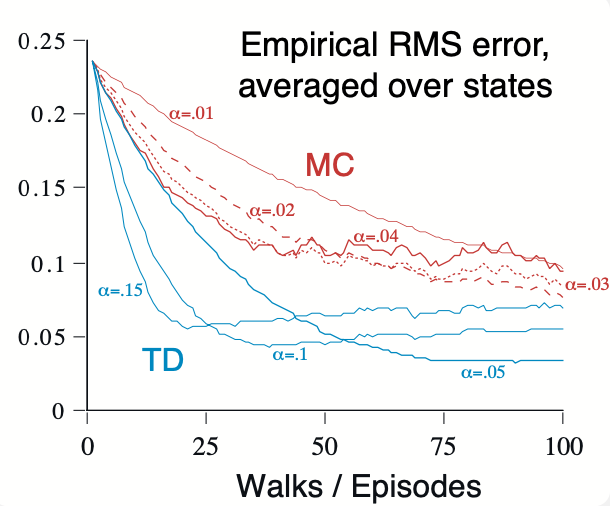
\includegraphics[width=0.5\textwidth]{images/td.png}
\end{figure}	

\end{frame}

\begin{frame}{Sarsa: on-policy TD Control}
\small
Similar to DP and Monte Carlo methods, we use the $Q$ function for the control problem, which implies the following update rule.
\begin{equation*}
	Q(s_t, a_t) \leftarrow Q(s_t, a_t) + \alpha \left[ r_t + \gamma Q(s_{t+1}, a_{t+1}) - Q(s_t, a_t)\right]
\end{equation*}

Notice that this time we require a tuple of $(s_t, a_t, r_t, s_{t+1}, a_{t+1})$, hence the name \textit{Sarsa}.
\end{frame}

\begin{frame}{Sarsa}
\small

\begin{algorithm}[H]
	\caption{Sarsa for estimating $Q^{\pi}$}
	Given any policy $\pi$, and specify step size parameters $\alpha \in (0, 1]$
	
	Initialize $Q^{\pi}(s, a) \forall s\in \mathcal{S}, a\in \mathcal{A}$
	
	\For{each episode}{
		Initialize $s$\;
		Choose action $a$ using policy derived from $Q$ (e.g. $\varepsilon$-greedy)\;
		
		\For{time step in this episode}{
		Take action $a$, observe $r, s'$\;
		Choose action $a'$ using policy derived from $Q$ (e.g. $\varepsilon$-greedy)\;
		
		$Q(s_t, a_t) \leftarrow Q(s_t, a_t) + \alpha \left[ r_t + \gamma Q(s_{t+1}, a_{t+1}) - Q(s_t, a_t)\right]$\;
		$s\leftarrow s', a\leftarrow a'$
		}
		}
\end{algorithm}

\end{frame}

\begin{frame}{Sarsa}
\small
\begin{itemize}[<+(1)->]
\item The convergence of Sarsa (in high probability) is guaranteed if \textbf{all} state-action pairs are visited an infinite number of times (thus we need exploration from a non-greedy policy) and $\varepsilon$-greedy converging to the greedy policy in the limit, for example by setting $\varepsilon = 1/t$.

\item Sarsa is hard to analyze. An early breakthrough in reinforcement learning is the development of the so-called \textit{Q-learning}, which leads to convergence proofs (some variants are proved very recently)
\item Notice a similar update rule of Sarsa can simplify the algorithm
$$ Q(s_t, a_t) \leftarrow Q(s_t, a_t) + \alpha \left[ r_t + \gamma \max_a Q(s_{t+1}, a) - Q(s_t, a_t)\right] $$
\end{itemize}
\end{frame}

\begin{frame}{Q-learning: Off-policy TD Control}
\footnotesize
Let's examine the update rule
$$ Q(s_t, a_t) \leftarrow Q(s_t, a_t) + \alpha \left[ r_t + \gamma \max_a Q(s_{t+1}, a) - Q(s_t, a_t)\right] $$

Now the $Q$ function directly approximates $Q^{\pi^*}$, the optimal action-value function, independent of the policy being followed. The resulting method thus is an \textit{off-policy} algorithm.

\begin{algorithm}[H]
	\caption{Q-learning for estimating $Q^{\pi}$}	
	\For{each episode}{
		Initialize $s$\;
		Choose action $a$ using policy derived from $Q$ (e.g. $\varepsilon$-greedy)\;
		
		\For{time step in this episode}{
		Take action $a$, observe $r, s'$\;
		
		$Q(s_t, a_t) \leftarrow Q(s_t, a_t) + \alpha \left[ r_t + \gamma \max_a Q(s_{t+1}, a) - Q(s_t, a_t)\right] $\;
		$s\leftarrow s'$
		}
		}
\end{algorithm}

\end{frame}

\begin{frame}{Q-learning}
\begin{itemize}
	\item Q-learning is a very successful algorithm. It remains important in the landscape of modern RL.
	\item Modification and variants have been proposed based on Q-learning. For example, Async Q-learning. 
	\item Deep Learning based RL methods rely heavily on the Q-learning update rule. But we will not introduce function approximation today.
\end{itemize}
\end{frame}

\begin{frame}{Expected Sarsa}
\small
Let's introduce one variant of Q-learning: expected Sarsa. The idea is to replace $\max$ operation with expected value based on current state.

\begin{equation*}
\begin{aligned}
Q\left(s_{t}, a_{t}\right) & \leftarrow Q\left(s_{t}, a_{t}\right)+\alpha\left[r_{t+1}+\gamma \mathbb{E}_{\pi}\left[Q\left(s_{t+1}, a_{t+1}\right) \mid s_{t+1}\right]-Q\left(s_{t}, a_{t}\right)\right] \\
&=Q\left(s_{t}, a_{t}\right)+\alpha\left[r_{t+1}+\gamma \sum \pi\left(a \mid s_{t+1}\right) Q\left(s_{t+1}, a\right)-Q\left(s_{t}, a_{t}\right)\right]
\end{aligned}
\end{equation*}

\begin{itemize}
	\item In expectation, Sarsa moves in the same direction as Expected Sarsa, hence the name.
	\item In some cases, Expected Sarsa is significantly better than Q-learning or Sarsa.
	\item Expected Sarsa subsumes and generalizes the two TD algorithms, but required additional computations. 
\end{itemize}
\end{frame}


\begin{frame}{Maximization Bias and Double Learning}
\small
\begin{itemize}
	\item In all TD control algorithms discussed, we take $\max$ over the estimated values. In this way, we implicitly use \textit{maximum of estimated values} as \textit{estimate of the maximum value}. This can lead to a significant positive bias.
	\item For example, for some state $s$, the true action-value function $Q(s, a)=0 $ for all $a$. But our current estimate $\widetilde{Q}(s, a)$ has some positive values and negative values. With the $\max$ operation, we implicitly over-estimate. Sutton calls this \textit{maximization bias}.
\item 
One way to view the problem is that it is due to using the same samples both to determine the maximizing action and to estimate values.
\item This bring the idea of \textit{Double Q-learning}, which maintains two $Q$ estimates $Q_1, Q_2$, and replace $\max_a Q_1(s', a)$ with $Q_1(s', \arg\max_a Q(s',a))$.
\end{itemize}
\end{frame}

\begin{frame}{Double Q-learning}
\small
\begin{algorithm}[H]
	\caption{Q-learning for estimating $Q^{\pi}$}	
	\For{each episode}{
		Initialize $s$\;
		Choose action $a$ using policy derived from $Q$ (e.g. $\varepsilon$-greedy)\;
		
		\For{time step in this episode}{
		Take action $a$, observe $r, s'$\;
		With 0.5 probability:\\ 
		$Q_1(s, a) \leftarrow Q_1(s, a) + \alpha \left[ r + \gamma  Q_1(s', \arg\max_a Q_2(s', a)) - Q_1(s, a)\right] $\;
		else:\\
		$Q_2(s, a) \leftarrow Q_2(s, a) + \alpha \left[ r + \gamma  Q_2(s', \arg\max_a Q_1(s', a)) - Q_2(s, a)\right] $\;
		$s\leftarrow s'$
		}
		}
\end{algorithm}
\end{frame}

\begin{frame}{Summary}
\begin{itemize}
	\item We introduced TD methods, which in spirit update our estimating using correction from steps ahead. 
	\item TD(0) for policy evaluation.
	\item Sarsa for on-policy control.
	\item Q-learning for off-policy control.
	\item Expected Sarsa, a generalized TD control method.
\end{itemize}
\end{frame}

\section{Ch7 $n$-step bootstrap}
\begin{frame}{$n$-step bootstrap}
\small
So far the key ingredients of tabular RL are represented. We introduce some new ideas with those methods. 

\begin{itemize}[<+(1)->]
	\item Instead of one-step look ahead in TD, estimate the TD target from $n$ steps followed. $$ V_{t+n}(s_t) \doteq V_{t+n-1}(s_t) + \alpha [G_{t:t+n} - V_{t+n-1}(s_t)]$$ where $G_{t:t+n} = r_{t+1}+\gamma r_{t+2} + \cdots + \gamma^n V_{t+n-1}(s_{t+n})$. 
	\item Same idea can be used for Sarsa and off-policy learning with importance sampling.
	\item $n$ step Q-learning, termed \textit{$n$ step Tree Backup}, achieves off-policy learning without importance sampling, by following the same recipe.
	\item Finally we can mix and match: take a convex combination of one-step target and $n$ step target.
\end{itemize}
\end{frame}

\section{Ch8 Planning and learning}
\begin{frame}{Planning and Learning}
\small
\begin{itemize}[<+(1)->]
	\item So far we discussed DP methods, which requires a model of the environment to learn; and Monte Carlo and TD methods, which are model-free methods that update estimation from current estimates.
	\item Humans learn things in both ways: we build a model based on our understandings, and simulate experience based on those model, we learn things from both simulated and real experiences.
	\item We can achieve the same goal by combining both types of methods.
\end{itemize}
\end{frame}

\begin{frame}{Dyna \cite{sutton2018reinforcement}}
\begin{figure}
	\centering
	\caption{The general Dyna Architecture. Real experience, passing back and forth between the environment and the policy, a↵ects policy and value functions in much the same way as does simulated experience generated by the model of the environment.}
	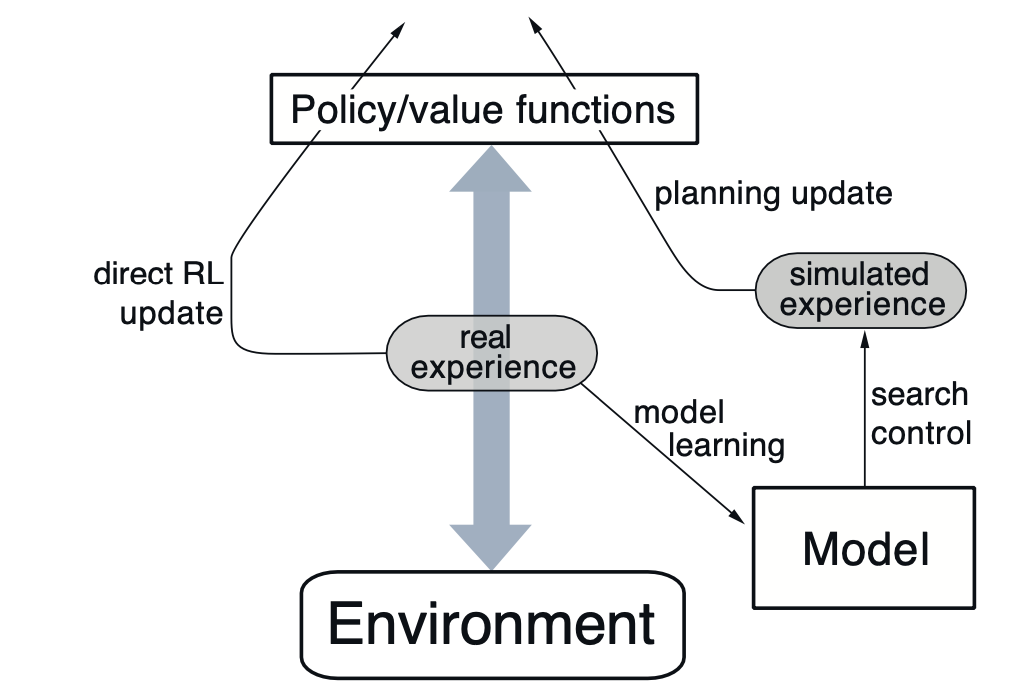
\includegraphics[width=0.8\textwidth]{images/planning.png}
\end{figure}
\end{frame}
%----------------------------%
% Conclusions

%\section{Summary}
%\begin{frame}{Summary }
%    \small
%    \begin{itemize}
%        \item
%    \end{itemize}
%\end{frame}

\begin{frame}
    \frametitle{}
    \centering
    
    \Large\color{gtblue}
    Thank you.

    \vspace{0.5cm}
    feiyangwu@gatech.edu

\end{frame}

%----------------------------%

% References slide
\begin{frame}[allowframebreaks]
\frametitle{References}
\footnotesize
\bibliographystyle{siam}
\bibliography{references} % bibliography file
\end{frame}

%%%%%%%%%%%%%%%%%%%%
\end{document}
%%%%%%%%%%%%%%%%%%%%
